% !TEX root = document.tex

\chapter{\label{chap:sdf3}WebDSL in SDF3}

  In computer science, parsing is the process of analyzing a piece of text according to a grammar, and converting the textual representation to a more structured representation that is convenient for other processes such as a compiler or interpreter.

  In this chapter we discuss the definition of the WebDSL grammar in SDF3, a meta-DSL in Spoofax for syntax definition. Currently, the WebDSL grammar is defined in SDF2, the predecessor of SDF3. The goal of defining the WebDSL grammar in SDF3 instead of SDF2 is to serve as a large case study for SDF3, while allowing the WebDSL parser to benefit from the regular updates of SDF3, compared to the deprecated SDF2.

  We start by giving a brief introduction to parsing in general and introducing the SDF3 language. Then, we discuss the migration of the WebDSL syntax from SDF2 to SDF3, and we end this chapter by elaborating on the disambiguation of the WebDSL SDF3 grammar without the use of post-parse filters.

  \section{\label{sec:parsing}Introduction to LR Parsing}

    Every programming language can be described by a grammar that specifies what a syntactically correct program looks like. Given a specific program, this grammar can be used to analyze whether the program belongs to the language described by the grammar. A parser is a piece of software that is able to recognize whether a program belongs to the grammar described by the parser. Additionally, parsers create a structured representation of the input program, derived from the textual representation.
    
    In this thesis, we will focus on \textit{LR parsers}. LR stands for Left-to-right Rightmost-derivation, meaning that an LR parser reads the input from left to right and produces a rightmost (bottom-up) derivation. Knuth \citeyear{knuth1965translation} presents an LR parsing algorithm which is able to parse most languages that can be described by a context-free grammar.

    Before an LR parser can parse an input stream, it must also receive a parse table that describes a context-free grammar. In practice, the parse tables are usually generated from a syntax definition. \Cref{fig:example-cfg-with-parse-table} shows an example of a context-free grammar describing a small language that features addition and multiplication. The parse table describes a push-down automaton that represents the LR parser. Using this parse table, an LR parser can build a parse tree as shown in \cref{fig:example-parse-tree}. A parse tree, or an Abstract Syntax Tree (AST) that we will discuss in \cref{subsec:sdf3} is a more structured way of representing a program, that can be used by other components of a compilation chain to analyze and transform the program.

    \begin{figure}[h]
      \begin{subfigure}[b]{0.25\textwidth}
        \centering
        \begin{align*}
        S &\longrightarrow E\\
        E &\longrightarrow E + T\\
        E &\longrightarrow T\\
        T &\longrightarrow T * F\\
        T &\longrightarrow F\\
        F &\longrightarrow x
        \end{align*}
        \caption{\label{fig:example-cfg-with-parse-table-cfg}}
      \end{subfigure}
      \begin{subfigure}[b]{0.75\textwidth}
        \centering
        \begin{tabular}{ c || c | c | c | c || c | c | c | c }
          State & \multicolumn{4}{c||}{Action} & \multicolumn{4}{c}{Goto} \\
          \hline
          & + & * & x & \$ & $S$ & $E$ & $T$ & $F$ \\
          \hline
          0 & & & $S(4)$ & & & 1 & 2 & 3 \\
          \hline
          1 & $S(5)$ & & & $Accept$ & & & & \\
          \hline
          2 & $R(E_T)$ & $S(6)$ & & $R(E_T)$ & & & & \\
          \hline
          3 & $R(T_F)$ & $R(T_F)$ & & $R(T_F)$ & & & & \\
          \hline
          4 & $R(F_x)$ & $R(F_x)$ & & $R(F_x)$ & & & & \\
          \hline
          5 & & & $S(4)$ & & & & 7 & 3 \\
          \hline
          6 & & & $S(4)$ & & & & & 8 \\
          \hline
          7 & $R(E_{E+T})$ & $S(6)$ & & $R(E_{E+T})$ & & & & \\
          \hline
          8 & $R(T_{T*F})$ & $R(T_{T*F})$ & & $R(T_{T*F})$ & & & & \\
        \end{tabular}
        \caption{\label{fig:example-cfg-with-parse-table-tbl}}
      \end{subfigure}
      \caption{\label{fig:example-cfg-with-parse-table}Example context-free grammar with its parse table}
    \end{figure}

    \begin{figure}
      \centering
      \begin{tikzpicture}
        \node {$S$}
          child {node {$E$}
            child {node {$T$}
              child {node {$T$}
                child {node {$F$}
                  child {node {$x$}}
                }
              }
              child {node {$*$}}
              child {node {$F$}
                child {node {$x$}}
              }
            }
          };
      \end{tikzpicture}
      \caption{\label{fig:example-parse-tree}An example of a parse tree for the input "$x * x$"}
    \end{figure}

    LR parsers cannot handle ambiguous context-free grammars. The parse tables of ambiguous context-free grammars contain multiple state transitions for certain states and input tokens. The Generalized LR (GLR) parsing algorithm by Rekers (\citeyear{Rekers1992}), is able to handle such parse tables and as a result is able to handle all context-free grammars. Visser \citeyear{Visser97SGLR} introduced Scannerless GLR (SGLR) parsing. As opposed to LR and GLR parsers, SGLR parsers do not have a separate lexing and parsing phase, but instead merge these through the use of grammars that are defined in terms of single characters.

    \subsection{\label{subsec:sdf3}SDF3}

      Syntax Definition Formalism 3 (SDF3) \autocite{VollebregtKV12,AmorimV20} is a meta-language in the Spoofax language workbench that makes use of the SGLR parsing algorithm. It is the latest version of the syntax definition formalism SDF \autocite{HeeringHKR89,Visser97}. Language engineers are able to define context-free grammars in SDF3, which are transformed into parse tables and used by the JSGLR2\footnote{\url{https://github.com/metaborg/jsglr}} parsing algorithm. JSGLR2 \autocite{Denkers2018} is the successor of the JSGLR algorithm; an implementation of the SGLR parsing algorithm in Java.

      SDF3 is the successor of SDF2, in which the WebDSL syntax is currently defined. Souza Amorim and Visser \citeyear{AmorimV20} argue that the SDF3 syntax is more similar to other grammar formalisms such as EBNF.

      A syntax definition in SDF3 is a declarative specification of syntactic sorts and their productions. \Cref{fig:sdf3-sorts-and-productions-syntax} shows an example grammar features a language that supports multiplication and addition of integers. The SDF3 definition must define a start-symbol that specifies what a syntactically valid program looks like. In our example, every program that can be derived from the \texttt{Start} sort, is a valid program. \textbf{Line 11} contains the first production of the specification. It states that the sort \texttt{Start} can be derived by deriving something of the sort \texttt{Expr}. The identifier behind the dot in the production (\texttt{Expr} in this case) declares the constructor in the AST. \Cref{fig:example-AST-1} shows the AST of an example input, according to the SDF3 specification of \cref{fig:sdf3-sorts-and-productions-syntax}. \textbf{Line 12-14} defines the productions of the expression sort. It defines that an expression is either two expressions with a plus or asterisk in between, or it is something of the sort \texttt{Lit}. The production of literal sort on \textbf{line 16} references the lexical sort \texttt{INT}. Lexical sorts do not appear in the AST with constructors, but instead are parsed into a string. The lexical sort \texttt{INT} is defined on \textbf{line 22} with the regular expression \texttt{[0-9]+}, describing one or more characters in the range of 0 to 9. Finally, the production describing the built-in concept of \texttt{LAYOUT} on \textbf{line 23} states that a space, tab, carriage return and line feed character are layout (whitespace) characters and do not have to be parsed.

      \Cref{fig:example-AST-1} shows the abstract syntax tree of an example input for the SDF3 specification of \cref{fig:sdf3-sorts-and-productions-syntax}. In the Spoofax Language Workbench, abstract syntax trees are described in the Annotated Terms Format (ATerm) \autocite{BrandJKO00}.

      \begin{figure}
        \begin{minted}[firstline=1]{\sdfthree}
  module ThesisTest

  context-free start-symbols
    Start

  context-free sorts
    Start Expr Lit

  context-free syntax
    Start.Expr = <<Expr>>

    Expr.Add = <<Expr> + <Expr>>
    Expr.Mul = <<Expr> * <Expr>>
    Expr.Lit = <<Lit>>

    Lit.Int = <<INT>>

  lexical sorts
    INT

  lexical syntax
    INT    = [0-9]+
    LAYOUT = [\ \t\n\r]
        \end{minted}
        \caption{\label{fig:sdf3-sorts-and-productions-syntax}An SDF3 specification of a language that allows addition and multiplication of integers.}
      \end{figure}

      \begin{figure}
        \begin{subfigure}[b]{0.5\textwidth}
          \centering
          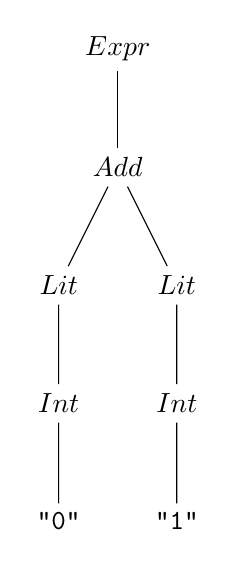
\begin{tikzpicture}
            \node {$Expr$}
              child {node {$Add$}
                child {node {$Lit$}
                  child {node {$Int$}
                    child {node {\texttt{"0"}}}
                  }
                }
                child {node {$Lit$}
                  child {node {$Int$}
                    child {node {\texttt{"1"}}}
                  }
                }
              };
          \end{tikzpicture}
          \caption{\label{fig:example-AST-1-ast}}
        \end{subfigure}
        \begin{subfigure}[b]{0.5\textwidth}
          \begin{minted}[firstline=1]{text}
Expr(
  Add(
    Lit(Int("0")),
    Lit(Int("1"))
  )
)
          \end{minted}
          \caption{\label{fig:example-AST-1-aterm}}
        \end{subfigure}
        \caption{\label{fig:example-AST-1}The AST and ATerm representation of the expression \texttt{0 + 1} according to the SDF3 specification of \cref{fig:sdf3-sorts-and-productions-syntax}}
      \end{figure}

      In addition to the basics as explained in the previous paragraph, SDF3 supports features such as injections, optional sorts and repetition to enhance the language engineers productivity. \cref{fig:sdf3-syntax-injection-repetition-optional} shows the SDF3 specification of \cref{fig:sdf3-sorts-and-productions-syntax}, but now enhanced with injections, repetition and optional sorts. \Cref{fig:example-aterm-injections-etc} shows the ATerm of the input \texttt{0 + 0; 1 * -1}. The repetition on \textbf{line x} of \cref{fig:sdf3-syntax-injection-repetition-optional} allows multiple expressions in a list, delimited by a semicolon. The injection on \textbf{line 14} allows a literal to be derived in the place of an expression, effectively omitting the \texttt{Lit(...)} constructor in the AST. Lastly, the optional minus sign of \textbf{line 16 and 18} allows negative integers to be parsed by this language. The AST contains \texttt{Some(...)} and \texttt{None()} constructors for the optional sorts.
        
      \begin{figure}
        \begin{minted}[firstline=1]{\sdfthree}
  module m

  context-free start-symbols
    Start
  
  context-free sorts
    Start Expr Lit Minus
  
  context-free syntax
    Start.Exprs = <<{Expr "; "}+>>
  
    Expr.Add = <<Expr> + <Expr>>
    Expr.Mul = <<Expr> * <Expr>>
    Expr     = Lit
  
    Lit.Int = <<Minus?> <INT>>
  
    Minus.Minus = <->
  
  lexical sorts
    INT
  
  lexical syntax
    INT    = [0-9]+
    LAYOUT = [\ \t\n\r]
        \end{minted}
        \caption{\label{fig:sdf3-syntax-injection-repetition-optional}An SDF3 specification of a language that allows addition and multiplication of integers, showcasing injections, repetition and optional sorts.}
      \end{figure}

      \begin{figure}
        \begin{minted}[firstline=1]{text}
  Exprs([
    Add(
      Int(None(), "0"),
      Int(None(), "0")
    ),
    Mult(
      Int(None(), "1")
      Int(Some(Minus()), "1")
    )
  ])
        \end{minted}
        \caption{\label{fig:example-aterm-injections-etc}The ATerm of input \texttt{0 + 0; 1 * -1} according to the SDF3 specification of \cref{fig:sdf3-syntax-injection-repetition-optional}}
      \end{figure}

      \subsubsection{\label{subsubsec:sdf3-disambiguation}Disambiguation}

        The simple grammar described by the SDF3 specification of \cref{fig:sdf3-sorts-and-productions-syntax} is functional, but is ambiguous. For example, the input \texttt{1 + 2 + 3} can be parsed as \texttt{(1 + 2) + 3} or as \texttt{1 + (2 + 3)}. The process of altering and annotating the grammar such that this there is only one way of parsing this, is called disambiguation. The example listed in the previous section (\cref{fig:example-cfg-with-parse-table}) contains a grammar with expressions, terms and factors that is inherently unambiguous. However, disambiguating a grammar by introducing new sorts and productions is tedious and time-consuming. SDF3 provides multiple options for disambiguating a grammar.

        First, SDF3 provides the \texttt{\{bracket\}} annotation, allowing the developer to disambiguate the program himself. To clarify, the input \texttt{1 + (2 + 3)} is not valid according to our grammar, because the "(" and ")" symbols are not part of the grammar. If we add the production \texttt{Expr = "(" Expr ")" \{bracket\}}, SDF3 allows brackets around arbitrary expressions without it introducing new AST nodes.

        Reject rules allow language engineers to filter derivations. A reject rule is simple a regular production, followed by the \texttt{\{reject\}} annotation. For example, appending our grammar with the rule \texttt{Expr = <<Expr> + <Expr>> \{reject\}} makes the set of valid derivations of \texttt{Expr} smaller, namely by disallowing any construction described by the right-hand side of the reject rule.

        Another possibility for disambiguating SDF3 grammars is by indicating the associativity, either as annotation or using priority groups. If we add the annotation \texttt{\{left\}} to the production that specifies addition, \texttt{1 + 2 + 3} is no longer ambiguous but instead will always be parsed as \texttt{(1 + 2) + 3}. It is also possible to declare the associativity in groups. \Cref{fig:sdf3-syntax-disambiguation} contains such groups. \textbf{Line 8} shows that both addition and subtraction are left associative, and in the same group. The input \texttt{1 + 2 - 3 + 4} will now be parsed as \texttt{((1 + 2) - 3) + 4}, whereas declaring the associativity annotation on both rules instead of the group would still make this input ambiguous.

        \begin{figure}
          \begin{minted}[firstline=2]{\sdfthree}
  module m
  context-free syntax
    Expr.Mul = <<Expr> * <Expr>>
    Expr.Add = <<Expr> + <Expr>>
    Expr.Sub = <<Expr> - <Expr>>

  context-free priorities
    {left: Expr.Mul} >
    {left: Expr.Add Expr.Sub }
          \end{minted}
          \caption{\label{fig:sdf3-syntax-disambiguation}An SDF3 specification of a simple language with disambiguation rules.}
        \end{figure}

        \Cref{fig:sdf3-syntax-disambiguation} also shows the declaration of priorities. In the example, multiplication has priority (e.g. binds tighter) over addition and subtraction. This results in the input \texttt{1 + 2 - 3 * 4} being parsed as \texttt{(1 + 2) - (3 * 4)}.

        SDF3 also provides the option of indexed priorities in the form of \texttt{p1 i .> p2}. This can be explained intuitively as the subterm with index \texttt{i} of production \texttt{p1} may not be derived by production \texttt{p2}. In our example, the rule \texttt{Expr.Add <0> .> Expr.Mul} would imply that the left-hand side of an addition may never be a multiplication.

        Lastly, SDF3 provides the ability to disambiguate through the use of post-parse filters annotated by \texttt{\{prefer\}} and \texttt{\{avoid\}}. When the parser encounters an ambiguous input, it will continue parsing and store all possibilities. At the end of parsing, it will use the annotations to prune the multiple ASTs according to these annotations. The \texttt{\{prefer\}} and \texttt{\{avoid\}} annotations are working but deprecated in the current version of SDF3 and will be removed in the future. Using the post-parse filters makes the disambiguation less transparent than using the other methods described in this section.

  \section{\label{sec:webdsl-grammar}WebDSL Grammar Specification}

    The current grammar of WebDSL is specified in SDF2, the predecessor of SDF3. Similar to SDF3, a production in the grammar consists of terminals and terminals. In contrast to SDF3, it is optional to provide a constructor to appear in the abstract syntax tree. \Cref{fig:sdf2-example} shows an example of productions in SDF2.

    \begin{figure}
      \begin{minted}[firstline=4]{\sdftwo}
module WebDSL-Action
exports
context-free syntax
  "var" Id ":" Sort ";"          -> VarDeclStat {cons("VarDecl")}
  "var" Id ":" Sort ":=" Exp ";" -> VarDeclStat {cons("VarDeclInit")}
  "var" Id ":=" Exp ";"          -> VarDeclStat {cons("VarDeclInitInferred")}
      \end{minted}
      \caption{\label{fig:sdf2-example}An example of productions in SDF2. This example specifies the syntax of variable declaration in WebDSL.}
    \end{figure}

    The WebDSL language SDF2 specification consists of 26 files that each describe a different part of the WebDSL syntax, ranging from the data model with entities to user interfaces with HTML and JavaScript. Additionally, the WebDSL syntax incorporates stand-alone grammars of other languages, such as HQL, Java and Stratego using mix syntax. Out of these mixed syntaxes, only the WebDSL and HQL syntax can be written by developers. The Java and Stratego syntax are used in other components of the WebDSL compiler, such as writing concrete WebDSL and Java syntax during desugaring, optimization and code generation.

    \subsection{Desugaring WebDSL Syntax}

      In WebDSL, the root of the abstract syntax tree is the application or module definition. A project is allowed to have one application and the other files should be modules that are (transitively) imported by the main application file.

      A file is divided in sections, which have no semantic meaning but are purely for code organization. The sections contain the top-level definitions such as pages, templates and entities. However, these sections are optional, and it is possible to list definitions without dividing them in sections.

      To prevent an explosion of cases in the analysis and code generation, these constructs are normalized (desugared) to a core WebDSL syntax. \Cref{fig:sdf2-sections} shows an example of desugaring different definitions of a file. 

      \begin{figure}
        \begin{subfigure}[b]{1\textwidth}
          \begin{minted}[firstline=3]{\sdftwo}
module WebDSL
exports
  context-free syntax
    "section" SectionName Definition*
      -> Section {cons("Section")}
    
    "application" QId Definition+ Section* 
      -> Application {cons("ApplicationDefs")}
    
    "application" QId Section*
      -> Application {cons("Application")}
          \end{minted}
          \caption{\label{fig:sdf2-sections-sdf}}
        \end{subfigure}
        \begin{subfigure}[b]{1\textwidth}
          \begin{minted}[firstline=3]{\stratego}
module WebDSL
strategies
  simplify-application-constructor :
    ApplicationDefs(qid, defs, sections)
      -> Application(qid, [Section("definitions", defs)|sections])
          \end{minted}
          \caption{\label{fig:sdf2-sections-stratego}}
        \end{subfigure}
        \caption{\label{fig:sdf2-sections}WebDSL Syntax and desugaring for sections and definitions}
      \end{figure}

  \section{\label{sec:sdf2-to-sdf3}Migration from SDF2 to SDF3}

    SDF2 is still supported by the Spoofax language workbench, but no longer actively developed. SDF3 is the most recent member of the Syntax Definitions Formalisms. In a sense, SDF3 is a high-level version of SDF2 with additional features. In the initial versions of SDF3, it compiled down to SDF2.

    Spoofax contains tool to migrate SDF2 specifications to SDF3 specifications but not all constructs of the lower level SDF2 are expressible in SDF3. The WebDSL SDF2 specification requires manual adjustment before this transformation tool can be utilized. Additionally, the generated SDF3 definition is suboptimal, as not all features of SDF3 are utilized in the generated code.

    \subsection{\label{subsec:preparing-webdsl-sdf2}Preparing the WebDSL SDF2 definition for migration}

      Not all SDF2 constructs can be expressed in SDF3. For this reason, the WebDSL SDF2 must be adjusted manually to be able to use the tool provided by Spoofax that transforms SDF2 specifications to SDF3 specifications.

      \paragraph{Sorts} Non-terminals are named \textit{Sorts} in SDF2 and SDF3. A production in SDF2 reduces a sequence of terminals and non-terminals to a certain sort, as listed in the example of \cref{fig:sdf2-sections}. In SDF2 the sort does not have to be declared in a separate \texttt{sorts} section, while it does in SDF3. Additionally, SDF2 does not differentiate lexical sorts from context-free sorts. The result of this difference in design is that SDF2 sorts cannot be migrated to SDF2, since the transformation tool does not know if an SDF2 sort is used as lexical or context-free sort. To be able to translate the SDF2 specification to SDF3, we must remove the sort declarations.

      \paragraph{Alternations} Another manual adjustment we must make to the SDF2 specification is removing alternations. An alternation is a production of the form \texttt{"a" | "b" -> S}. This construct is not supported anymore in SDF3 and therefore the transformation tool is not able to handle this construct. Fortunately, the alternation can easily be split in two production rules. However, the transformation tool does not automate this process because the original production may contain a constructor annotation (\texttt{"a" | "b" -> S \{cons("AorB")\}}) and the duplicate constructors for the same sort are not allowed in SDF3. For this reason must manually remove alternations in SDF2 productions.

      \paragraph{Follow Restrictions} The transformation tool does also not include support for follow restrictions in the grammar. A follow restriction indicates what symbols are not allowed to be parsed after a production. A typical use case of this is ensuring the longest match for identifiers, or enforcing whitespace after a keyword. An example of follow restrictions are shown in \cref{fig:sdf2-follow-restrictions}. For the migration to SDF3, these sections have to be manually copied.

      \begin{figure}
        \begin{minted}[firstline=3]{\sdftwo}
module x
exports
  lexical syntax
    [a-zA-Z\_][a-zA-Z0-9\_]* -> ID
  lexical restrictions
    ID -/- [a-zA-Z0-9\_]
    "in" -/- [a-zA-Z0-9\_]
        \end{minted}
        \caption{\label{fig:sdf2-follow-restrictions}Follow restrictions are used to for example ensure the longest-match of an identifier and enforcing whitespace after keywords.}
      \end{figure}

    \subsection{\label{subsec:manual-tweaking-sdf3}Manual Adjustment of Generated WebDSL SDF3}

      The generated SDF3 specification of WebDSL according to the manually adjusted SDF2 is suboptimal SDF3 code. SDF2 can be seen as a more low-level version of SDF3 and not all constructs of SDF2 transform into the most elegant SDF3 code. Parts of the generated SDF3 code do not even adhere to the static semantics of SDF3. For this reason, the generated SDF3 code has to be manually adjusted.

      \paragraph{Missing and duplicate constructors} In SDF2, constructors are defined as an annotation on a production. An example of the different production syntax of SDF2 and SDF3 is shown in \cref{fig:sdf2-sections}. The constructor annotation is not required in SDF2, but in SDF3 it is necessary to provide a constructor for every production. In the WebDSL SDF2 definition, some constructors are missing and there were are duplicate constructors that denoted alternative syntax for the same construct, essentially providing syntactic sugar. The SDF2 definition and generated SDF3 definition for the \texttt{ascending} and \texttt{descending} ordering is shown in \cref{fig:sdf2-sdf3-asc-desc}.

      \begin{figure}
        \begin{subfigure}[b]{1\textwidth}
          \begin{minted}[firstline=3]{\sdftwo}
module WebDSL-UI
exports
  context-free syntax
    "asc"        -> AscendingOrDescending {cons("Ascending")}
    "ascending"  -> AscendingOrDescending {cons("Ascending")}
    
    "desc"       -> AscendingOrDescending {cons("Descending")}
    "descending" -> AscendingOrDescending {cons("Descending")}
          \end{minted}
          \caption{\label{fig:sdf2-sdf3-asc-desc-sdf2}}
        \end{subfigure}
        \begin{subfigure}[b]{1\textwidth}
          \begin{minted}[firstline=2]{\sdfthree}
module WebDSL-UI
  context-free syntax
    HQLAscOrDescOpt.HQLAscending = <ascending>
    HQLAscOrDescOpt.HQLAscending = <asc>   // Error: duplicate constructor

    HQLAscOrDescOpt.HQLDescending = <descending>
    HQLAscOrDescOpt.HQLDescending = <desc> // Error: duplicate constructor
          \end{minted}
          \caption{\label{fig:sdf2-sdf3-asc-desc-sdf3}}
        \end{subfigure}
        \caption{\label{fig:sdf2-sdf3-asc-desc}SDF2 and generated SDF3 for the \texttt{ascending} and \texttt{descending} keyword in WebDSL. Duplicate constructors within the same sort are not allowed in SDF3.}
      \end{figure}
      
      In the newly generated SDF3, duplicate constructors must be changed, in order for them to be unique. Additionally, missing constructors must be added for the pretty-printer to function correctly. Injections do typically not require a constructor, but preferably constructors should be added there as well to reduce the length of the abstract syntax tree in Statix, as we will explain in \cref{sec:preparation-for-statix}.

      \paragraph{Priority chains} Priority chains are used to disambiguate grammars in SDF specifications. A typical example and an explanation is given in \cref{fig:sdf3-syntax-disambiguation}. Both SDF2 and SDF3 use the concept of priority chains, but the SDF2 variant requires a repetition of the production inside the chain, whereas SDF3 uses a reference to the production. This causes the SDF2 priority chains to not be migrated to the SDF3 priority chains and requires them to be manually rebuilt. An example of the difference between priority chains in SDF2 and SDF3 is shown in \cref{fig:sdf2-sdf3-asc-priority-chains}.

      \begin{figure}
        \begin{subfigure}[b]{0.5\textwidth}
          \begin{minted}[firstline=3]{\sdftwo}
module WebDSL-UI
exports
  context-free priorities
    {left:
      Expr "*" Expr -> Expr
    } >
    {left:
      Expr "+" Expr -> Expr
      Expr "-" Expr -> Expr
    }
          \end{minted}
          \caption{\label{fig:sdf2-sdf3-asc-priority-chains-sdf2}}
        \end{subfigure}
        \begin{subfigure}[b]{0.5\textwidth}
          \begin{minted}[firstline=2]{\sdfthree}
module WebDSL-UI
context-free priorities
  {left: Expr.Mul} >
  {left: Expr.Add Expr.Sub }
          \end{minted}
          \caption{\label{fig:sdf2-sdf3-asc-priority-chains-sdf3}}
        \end{subfigure}
        \caption{\label{fig:sdf2-sdf3-asc-priority-chains}Difference between priority chains in SDF2 and SDF3. The transformation tool does not perform the analysis to properly transform this.}
      \end{figure}

      \paragraph{Transferring comments} Comments are highly recommended and important for the readability and maintainability of large software projects. However, most grammars specified in SDF2 and SDF3 declare comments as part of the layout of a program and are not represented in the abstract syntax tree. For this reason, the transformation tool does not transfer comments from SDF2 grammars to the generated SDF3. Comments must be manually copied from the SDF3 and pasted in the correct parts of the SDF3 specification.

      \paragraph{Template productions} A major change in SDF3 compared to SDF2 are template productions, that allow for nice pretty printing and syntactic code completion. The productions in the generated SDF3 files are all template productions, but do not have the proper surrounding layout and indentation because there is no way to extract this information from the SDF2 source, as it is not present there. Adding the correct layout in template productions is tedious work but causes the pretty-printer to function properly. An example of SDF2, generated SDF3 and manually adjusted SDF3 is shown in \cref{fig:sdf2-sdf3-template-production}.

      \begin{figure}
        \begin{subfigure}[b]{1\textwidth}
          \begin{minted}[firstline=3]{\sdftwo}
module WebDSL-UI
exports
  context-free syntax
    "if" "(" Expr ")" "{" Expr* "}" -> Expr {cons("If")}
          \end{minted}
          \caption{\label{fig:sdf2-sdf3-template-production-sdf2}}
        \end{subfigure}
        \begin{subfigure}[b]{0.6\textwidth}
          \begin{minted}[firstline=2]{\sdfthree}
module WebDSL-UI
  context-free syntax
    Expr.If = <if ( <Expr> ) { <Expr*> }>
          \end{minted}
          \caption{\label{fig:sdf2-sdf3-template-production-sdf3-gen}}
        \end{subfigure}
        \begin{subfigure}[b]{0.4\textwidth}
          \begin{minted}[firstline=2]{\sdfthree}
module WebDSL-UI
  context-free syntax
    Expr.If = <
      if ( <Expr> ) {
        <Expr*> 
      }
    >
          \end{minted}
          \caption{\label{fig:sdf2-sdf3-template-production-sdf3-adjusted}}
        \end{subfigure}
        \caption{\label{fig:sdf2-sdf3-template-production}An example of an SDF2 production, the generated SDF3 and the manually adjusted SDF3 for template productions.}
      \end{figure}

      \paragraph{Deeply Embedding HQL Grammar in WebDSL} The HQL syntax definition in SDF2 is a stand-alone definition, and is used in the WebDSL SDF2 using parameterized imports. SDF3 has no support for this feature, which means the syntax definition has to be transformed to be a part of the WebDSL grammar. Otherwise, WebDSL applications that use HQL syntax, which are all real world applications, would no longer parse correctly. Deeply embedding the HQL syntax in the WebDSL syntax causes sorts and constructors to overlap, and this must be adjusted manually.

  \section{\label{sec:preparation-for-statix}Preparation for Statix}

    Statix is a constraint-based meta-language in which we implement the modernized WebDSL static analysis. In \cref{chap:statix} Statix will be explained in detail. Even though the parsing and the static analysis are separate components of the compilation chain, the Spoofax language workbench contains a tool that extracts the sorts and constructors from an SDF3 definition, and generates these signatures in the Statix language to be able to use them while defining the static analysis. This tool is called the Statix signature generator. Using the Statix signature generator imposes additional constraints on the SDF3 definition.

    \subsection{\label{subsec:sorts-in-statix}Sorts and Constructors in Statix}

      To understand the role of the Statix signature generator, we will explain how sorts and constructors are used in Statix to define the static semantics of a language.

      Unlike SDF3 and Stratego, Statix is strongly typed which requires all sorts and constructors to be declared before they can be used in the static semantics of a language. \Cref{fig:statix-expression-language} shows an example of declaration of the sorts and constructors of a simple expression language. These constructors and terms can be used in rules that form the static semantics.

      \begin{wrapfigure}{r}{0.58\linewidth}
        % \vspace{-15pt}
        \capstart
        \begin{minted}[]{\statix}
  module x
  signature
    sorts
      Application
      Expr
    
    constructors
      Application : Expr        -> Application
      Add         : Expr * Expr -> Expr
      Sub         : Expr * Expr -> Expr
      Mul         : Expr * Expr -> Expr
      Int         : string      -> Expr
        \end{minted}
        \caption{\label{fig:statix-expression-language}An example of an expression language signature in Statix.}
        % \vspace{-10pt}
      \end{wrapfigure}

      The constructors in Statix do not support injections or overloaded constructors, which leaves some abstract syntax trees generated by the parser unable to serve as input for static analysis.

    \subsection{\label{subsec:statix-signature-generator}Statix Signature Generator}

      As mentioned and demonstrated in the previous subsection, Statix requires a definition of the constructors and sorts of the language to be analyzed. Defining these manually in Statix would essentially be code duplication because they are already defined in SDF3. However, Statix sorts and constructors do not support overloading and injections and is therefore stricter than the SDF3 type system.

      To prevent manual redefinition of the sorts in Statix code, the Statix signature generator is part of Spoofax. This tool takes an SDF3 definition as input, and generates importable Statix files that contain the sorts and constructors from the syntax definition. For the Statix signature generator to work properly, Additional constraints are imposed on the SDF3 definition.

      \paragraph{Explicitly Declare Sorts} To define static semantics of all sorts in a language, these must be explicitly declared in Statix. In SDF3 this is not enforced. To be able to use the Statix signature generator, we have to explicitly declare all sorts in the WebDSL SDF3. Additionally, Statix views all lexical sorts as strings, so the SDF3 sorts have to be divided in lexical sorts and context-free sorts.

      \paragraph{Injections} With the semantics of sorts and constructors in Statix, it is not possible to model injections while the WebDSL SDF3 definition contains many injections. The Statix signature generator still functions with injections present in the SDF3, but it will generate an additional constructor and \textit{explicate} the constructors of an abstract syntax tree before it is passed to Statix. \Cref{fig:sdf3-statix-explication} shows an example of how injections are handled an explicated by the Statix signature generator. The abstract syntax tree is explicated after parsing and before static analysis. When injections are present in the SDF3, the Statix signature generator also generates Stratego rules that explicate the abstract syntax tree.

      \begin{figure}
        \begin{subfigure}[b]{0.5\textwidth}
          \begin{minted}[firstline=2]{\sdfthree}
module WebDSL-UI
  context-free sorts
    S A B
  context-free syntax
    S.Start   = A
    A         = B // injection
    B.Literal = "b"
          \end{minted}
          \caption{\label{fig:sdf3-statix-explication-sdf3}SDF3}
        \end{subfigure}
        \begin{subfigure}[b]{0.5\textwidth}
          \begin{minted}[]{\statix}
module x
signature
  sorts
    S A B
  
  constructors
    Start   : A -> S
    Literal :      B
    // extra generated constructor
    B2A     : B -> A
          \end{minted}
          \caption{\label{fig:sdf3-statix-explication-statix}Generated Statix signatures}
        \end{subfigure}
        \begin{subfigure}[b]{0.5\textwidth}
          \begin{minted}[firstline=1]{text}
  Start(
    Literal()
  )
          \end{minted}
          \caption{\label{fig:sdf3-statix-explication-ast}Example of an AST}
        \end{subfigure}
        \begin{subfigure}[b]{0.5\textwidth}
          \begin{minted}[firstline=1]{text}
  Start(
    B2A(
      Literal()
    )
  )
          \end{minted}
          \caption{\label{fig:sdf3-statix-explication-explicated}Example of an explicated AST}
        \end{subfigure}
        \caption{\label{fig:sdf3-statix-explication}An example of how SDF3 injections are handled by the Statix signature generator.}
      \end{figure}

      \paragraph{\label{par:optional-sorts}Optional Sorts} As mentioned in \cref{fig:sdf3-syntax-injection-repetition-optional} as part of \cref{subsec:sdf3}, SDF3 has built-in support for optional sorts, resulting in \texttt{Some(\_)} and \texttt{None()} terms. These terms cannot be  translated to Statix signatures, since it is not possible to overload the constructor for many sorts. To work around this limitation, the SDF3 definition must be altered make the \texttt{Some} and \texttt{None} constructors unique per sort. This leads to a much more verbose syntax definition. \Cref{fig:sdf3-remove-optionals} shows how the optional constructs can be altered to be unique per sort.

      \begin{figure}
        \begin{subfigure}[b]{1\textwidth}
          \begin{minted}[firstline=2]{\sdfthree}
module WebDSL-UI
  context-free syntax
    Definition.Function = <
      function <ID> () <ReturnSort?> {
        <Statement*>
      }
    >

    ReturnSort.ReturnSort = <: <Sort>>
          \end{minted}
          \caption{\label{fig:sdf3-remove-optionals-before}SDF3 with optionals}
        \end{subfigure}
        \begin{subfigure}[b]{1\textwidth}
          \begin{minted}[firstline=2]{\sdfthree}
module WebDSL-UI
  context-free syntax
    Definition.Function = <
      function <ID> () <ReturnSortOpt> {
        <Statement*>
      }
    >

    ReturnSortOpt.ReturnSort     = <: <Sort>>
    ReturnSortOpt.ReturnSortNone = <>
          \end{minted}
          \caption{\label{fig:sdf3-remove-optionals-after}Rewritten to remove optionals}
        \end{subfigure}
      \caption{\label{fig:sdf3-remove-optionals}An example of how to remove the optional sort to comply with the Statix signature generator.}
      \end{figure}

      \paragraph{Disambiguation} SDF3 provides many features to disambiguate a grammar as listed in \cref{subsubsec:sdf3-disambiguation}. If an ambiguous code fragment is parsed, it will result in the \texttt{amb([...])} term in the AST, which contains a list of the possible interpretations. Similar to the \texttt{Some(\_)} and \texttt{None())} constructors from the optionals as discussed in the previous paragraph, the \texttt{amb([...])} can not be expressed in Statix. The result of this is that ambiguous code fragments can not be used in Statix rules and therefore will never be analyzed, increasing the need for proper disambiguation even more. In the next section we will discuss the disambiguation of the WebDSL SDF3 grammar.

  \section{\label{sec:webdsl-sdf3-disambiguation}Disambiguation}
  
    When a program is ambiguous, it can be interpreted in multiple ways. Generally, ambiguous programs are undesired due to the undefined semantics. To prevent ambiguities in the syntax of a programming language, the syntax definition can be disambiguated.

    SDF3 provides multiple language features to disambiguate a syntax, such as bracket rules, reject rules, associativity annotations, priority groups and indexed priorities. A complete list of ways to disambiguate is explained in \cref{subsubsec:sdf3-disambiguation}.

    Post-parse filters \texttt{\{prefer\}} and \texttt{\{avoid\}} provide a unique way to disambiguate the syntax, namely it keeps all the possible parse trees in memory and after the whole input is parsed, the parser prunes the resulting parse forest according to the \texttt{\{prefer\}} and \texttt{\{avoid\}} annotations.
    
    The \texttt{\{prefer\}} and \texttt{\{avoid\}} post-parse filters are deprecated in the current version of SDF3. In this thesis we attempt to disambiguate the grammar of a WebDSL with the other disambiguation functionalities provided by SDF3.

    \subsection{Disambiguating Keywords}

      WebDSL template calls do not require parentheses or semicolons. This allows for clean code in templates, but makes the syntax ambiguous in the case of keywords that are able to parse as a template name.
      
      \Cref{fig:sdf3-keywords-ambiguous} shows an example of a WebDSL program where a template starts with a variable initialization with an HQL query that fetches all names of users from the database. In HQL, the from-clause is optional, meaning that a statement such as \texttt{select user.name} syntactically correct as an HQL expression. For this reason, the words after the select clause can also be parsed as template calls.

      \begin{figure}
        \begin{minted}[firstline=2]{\webdsl}
module x
  template t() {
    // from-clause is optional in this HQL expression
    // meaning that "select u.name" is a complete expression
    // and "from", "User", "as", and "u" can also be parsed
    // as template calls
    var names := select u.name from User as u

    // parentheses are optional in template calls
    callToOtherTemplate
  }
        \end{minted}
        \caption{\label{fig:sdf3-keywords-ambiguous}An example of an ambiguous construct in WebDSL with an HQL query.}
      \end{figure}

      A simple yet effective solution is to disallow all keywords such as \texttt{from} and \texttt{as} from being valid template names. SDF3 automatically detects keywords from context-free productions, and all keywords can be rejected as identifiers at once using template options\footnote{\url{https://www.spoofax.dev/references/syntax/templates/\#reject}}. An example of how keyword rejection in template options is configured, is shown in \cref{fig:sdf3-template-options-reject}.

      \begin{figure}
        \begin{minted}[firstline=2]{\sdfthree}
module x
  lexical syntax
    ID = [a-zA-Z]*

  context-free syntax
    Start.Hello = <hello <Name>>

    Name.World = <world>
    Name.Name = <<ID>>

  template options
    // "hello" and "world" are now no longer valid IDs
    ID = keyword {reject}
        \end{minted}
        \caption{\label{fig:sdf3-template-options-reject}An example of rejecting keywords in template options.}
      \end{figure}

      Rejecting all keywords in the WebDSL language using the template options of SDF3 would be effective, but too rigorous. For example, the WebDSL grammar contains productions such as the following. Rejecting all keywords would imply also rejecting \texttt{Int} as identifier, meaning that it is now allowed as type anymore.
      
      \texttt{Statement.ForCountStmt = <for ( <VarId> : Int from <Exp> to <Exp> ) <Block>>}

      Another option is to add all the reject rules for keywords individually. This is tedious work, but allows for better precision. In the new WebDSL SDF3, all keywords are rejected individually.

    \subsection{Disambiguating Strings}

      WebDSL strings are defined in SDF2 using kernel syntax. Kernel syntax does not allow implicit layout (whitespace) between the different elements of a production. The SDF2 productions for a WebDSL string are shown in \cref{fig:sdf2-webdsl-string}. A string can be either a "simple" string or a string containing one or more expressions that have to be evaluated. These expressions must be prefixed by a tilde (\texttt{~}) to be parsed as interpolation.

      \begin{figure}
        \begin{minted}[firstline=3]{\sdftwo}
module x
exports
  %% Kernel syntax is required here since we do not want LAYOUT to be parsed
  %% between the first QMLex and StringLex
  syntax
    %% string literal as expression
    <QMLex-LEX> <StringLex-LEX> <QMLex-LEX>
      -> <String-CF> {ast("String(<2>)")}

    <QMLex-LEX> StringPart* <QMLex-LEX>
      -> <String-CF> {ast("StringInterp(<2>)"), avoid}

    SimpleStringPart       -> StringPart
    <StringLexInterp-LEX>  -> StringPart

    "~" <SimpleExp-CF>    -> SimpleStringPart {cons("InterpExp")}
    "~" "(" <Exp-CF> ")"  -> StringPart {cons("InterpExp")}
        \end{minted}
        \caption{\label{fig:sdf2-webdsl-string}SDF2 definitions of a WebDSL string.}
      \end{figure}

      To prevent a simple string from being parsed as a \texttt{StringInterp} with only one part, the SDF2 definition used a post-parse filter to avoid this construct in case of ambiguities.
      
      \Cref{fig:sdf3-webdsl-string} shows the SDF3 definition of a WebDSL string. The "simple" string constructor was dropped, to ensure no ambiguity would arise. A simple string is now a string consisting of only one part.

      \begin{figure}
        \begin{minted}[firstline=2]{\sdfthree}
module x
  // Kernel syntax is required here since we do not want LAYOUT to be parsed
  // between the first quote and StringLex
  syntax

    String-CF.String = "\"" StringPart-CF* "\""

    StringPart-CF.StringValue = StringLex-LEX
    StringPart-CF.InterpValue = "~" StringInterpExp-CF
    StringPart-CF.InterpExp = "~" "(" Exp-CF ")"

    StringInterpExp-CF.InterpSimpleExp = SimpleExp-CF
        \end{minted}
        \caption{\label{fig:sdf3-webdsl-string}SDF3 definitions of a WebDSL string.}
      \end{figure}

    \subsection{Non-transitive Priority Rules}

      Another ambiguity in the WebDSL language is the overlap between passing template elements and the untyped set creation. \Cref{fig:sdf3-webdsl-untyped-set} demonstrates the ambiguity. The curly brackets are used for an untyped set creation, as shorthand for \texttt{Set<Int>(...)}. On the other hand, curly brackets are also used to pass template elements as argument to another template.

      \begin{figure}
        \begin{minted}[firstline=2]{\webdsl}
module x
  page p() {
    var mySet := { 1, 2, 3 } // untyped set creation

    t({ "Hello World" }) // pass template elements as argument
  }

  template t(elems : TemplateElements) {
    elems // this will render the content of elems
  }
        \end{minted}
        \caption{\label{fig:sdf3-webdsl-untyped-set}Ambiguous WebDSL code using curly brackets for untyped set creation and passing template elements as argument.}
      \end{figure}

      In SDF3, indexed non-transitive priorities are able to disambiguate this case. An indexed non-transitive priority rule is of the form \texttt{SortA.ConsA <n> .> SortB.ConsB}. Intuitively, the rule indicates that \texttt{SortB.ConsB} may never be the $n$-th subterm of \texttt{SortA.ConsA}. \Cref{fig:sdf3-non-transitive-priorities} shows how the WebDSL syntax can be disambiguated using these priorities.

      \begin{figure}
        \begin{minted}[firstline=2]{\sdfthree}
module x
  context-free syntax
    Exp.UntypedSetCreation = <{ <{Exp ","}+> }>

    TemplateArg.TemplateArgExp = <<Exp>>
    TemplateArg.TemplateArgElements = <{ <TemplateElements*> }>

  context-free priorities
    TemplateArg.TemplateArgExp <0> .> Exp.UntypedSetCreation
        \end{minted}
        \caption{\label{fig:sdf3-non-transitive-priorities}Using non-transitive indexed priorities to disambiguate WebDSL syntax in SDF3.}
      \end{figure}

      Another instance of an ambiguity that is corrected with indexed non-transitive priority rules is optional type aliases versus a cast expression. WebDSL allows a switch-case statement on the type of an expression. \Cref{fig:sdf3-webdsl-typecase} shows an example of how it is used in WebDSL code. The typecase takes an expression as subterm, and an optional type alias. The type alias automatically is the expression cast to whatever case is relevant. However, the expression given to the typecase can also be a cast expression, making \texttt{typecase(e as t)} ambiguous.

      \begin{figure}
        \begin{minted}[firstline=2]{\webdsl}
module x
  template t(e : Entity) {
    // example of a cast expression
    var x := e as User

    // switch-case statement on the type of a variable
    typecase(e) {
      User    { "e is a User"     showUser(e as User)      }
      Student { "e is a Student"  showStudent(e as Student)}
      default { }
    }

    // switch-case statement on the type of a variable using an alias
    // the alias automatically casts the expression based on the case
    typecase(e as t) {
      User    { "e is a User"     showUser(t)   } // t := e as User
      Student { "e is a Student"  showStudent(t)} // t := e as Student
      default { }
    }
  }
        \end{minted}
        \caption{\label{fig:sdf3-webdsl-typecase}Ambiguous WebDSL code using an optional typecase alias or a cast expression.}
      \end{figure}

      \Cref{fig:sdf3-typecase-disambiguation} shows how the optional type alias versus a cast expression is disambiguated in the modernized WebDSL SDF3 definition. The index of the \texttt{<Exp>} subterm is 2 and not 0 because the index counts literals as well, \texttt{typecase} and \texttt{(} in this case.

      \begin{figure}
        \begin{minted}[firstline=2]{\sdfthree}
module x
  context-free syntax
    Exp.Cast = <<Exp> as <Sort>>
    Statement.TypeCaseStmt = <
      typecase ( <Exp> <OptTypeAlias> ) {
        <TypeCaseAlt*>
      }
    >
    OptTypeAlias.TypeAlias = <as <Id>>
    OptTypeAlias.OptTypeAliasNone = <>

  context-free priorities
    Statement.TypeCaseStmt <2> .> Exp.Cast
        \end{minted}
        \caption{\label{fig:sdf3-typecase-disambiguation}Using non-transitive indexed priorities to disambiguate WebDSL casts versus type aliases.}
      \end{figure}
